\chapter{Simulation, Reconstruction and Event Selections}
\label{chap:Selections}

\section{Simulation}
\label{sec:Selections_Simulation}

In order to generate a Monte Carlo prediction of the expected event rate at the far detector for both sets of samples, all the processes in the beamline, atmospheric flux, neutrino interaction and detector need to be modelled. The beamline simulation consists of three distinct parts; initial hadron interaction modelling, target station geometry and particle tracking and hadronic re-interactions. These are modelled by FLUKA \cite{fluka2011}, JNUBEAM \cite{geant3, PhysRevD.87.012001} and GCALOR \cite{gcalor}, respectively. FLUKA is not very adaptable but matches external cross-section measurements in the region of interest better than GCALOR (\quickmath{O(10)\text{GeV}}). Thus a small simulation is built to model the interactions in the target and the output is then passed to JNUBEAM and GCALOR for propagation. The hadronic interactions are tuned to data from the NA61/SHINE \cite{Abgrall_2011, Abgrall_2012, NA61_pions_rep} and HARP \cite{harp} experiments. The tuning is done by reweighting the FLUKA and GCALOR predictions to match the external data multiplicity and cross-section measurements, based on final state particle kinematics \cite{t2k_tn_flux}. The predicted flux for neutrino and antineutrino beam modes is illustrated in \autoref{fig:T2KSKExp_T2K_NuFluxPerMode}.

The atmospheric neutrino flux predictions are simulated by the HKKM model \cite{Honda_2007, Honda:2011}, where the primary cosmic ray flux is tuned to AMS \cite{Blau2002} and BESS \cite{Haino2004} external data assuming the US-standard atmosphere `76 \cite{USStandardAtm} density profile and includes geomagnetic field effects. Secondary interactions of pions and muons are handled by DPMJET-III \cite{Roesler2001} for energies above \quickmath{32\text{GeV}} and JAM \cite{Niita2006, Honda:2011} for energies below that value. These hadronic interactions are tuned to external data \cite{Sanuki_2002, Achard_2004} using the same methodology as the tuning of the beamline simulation. The energy and cosine zenith predictions of \quickmath{\nu_{e}, \bar{\nu}_{e}, \nu_{\mu}, \bar{\nu}_{\mu}} flux are given in \autoref{fig:NeutrinoOscillationPhysics_AtmosphericNeutrinoFlux} and \autoref{fig:NeutrinoOscillationPhysics_NuFluxZenithAngleDep}, respectively. The flux is approximately symmetrical and peaked around \quickmath{\cos(\theta_{Z}) = 0.0}. This is because horizontally-going pions and kaons can travel further than their vertically-going counterparts resulting in a larger probability of decay to neutrinos. The symmetry is broken in low-energy neutrinos due to geomagnetic effects, which modify the track of the primary cosmic rays.

The neutrino interactions in all three detectors are simulated with NEUT \cite{Hayato2021, neut}. This simulates quasi-elastic (QE), meson exchange (MEC), single meson production (PROD), coherent pion production (COH) and deep inelastic scattering (DIS) interactions. These interaction categories can be further broken down by whether they were propagated via a \quickmath{W^{\pm}} boson in Charged Current (CC) interactions or via a \quickmath{Z^{0}} boson in Neutral Current (NC) interactions. CC interactions have a charged lepton in the final state, which can be flavour-tagged in reconstruction to determine the flavour of the neutrino. In contrast, NC interactions have a neutrino in the final state so no flavour information can be determined from the observables in the detector. This is the reason why NC events are assumed to not oscillate within the analysis. Both CC and NC interactions are modelled for all the above interaction categories, other than MEC interactions which are only modelled for CC events. The SK detector is only sensitive to charged particles, so all charged current interactions are simulated whilst only neutral current processes which produce charged mesons (NCDIS, NCCOH and NCPROD) are modelled. NC MEC interactions can only produce charged particles through secondary re-interactions which is a low cross-section process.

\begin{figure}[h]
  \begin{subfigure}[t]{0.8\textwidth}
    \includegraphics[width=\textwidth, trim={0mm 0mm 0mm 0mm}, clip,page=1]{Figures/Selections/NEUTCrossSection.pdf}
  \end{subfigure}
  \caption{The NEUT prediction of the \quickmath{\nu_{\mu}}-H2O cross-section overlaid on the T2K \quickmath{\nu_{\mu}} flux. The charged current (black, solid) and neutral current (black, dashed) inclusive, charged current quasi-elastic (blue, solid), charged current 2p2h (blue, dashed), charged current single pion production (pink) and charged current multi--\quickmath{\pi} and DIS (Purple) cross-sections are illustrated. Taken from \cite{Hayato2021}.}
  \label{fig:Selection_CrossSection}
\end{figure}

As illustrated in \autoref{fig:Selection_CrossSection}, QE interactions dominate the low-energy cross-section of neutrino interactions. The NEUT implementation adopts the Llewellyn Smith \cite{llewelyn-smith} model for neutrino-nucleus interactions, where the nuclear ground state of any bound nucleons (neutrino-oxygen interactions) is approximated by a spectral-function \cite{Benhar1989} model that simulates the effects of Fermi momentum and Pauli blocking. The cross-section of QE interactions are controlled by vector and axial-vector form factors parameterised by the BBBA05 \cite{bbba05} model and a dipole form factor with \quickmath{M_{A}^{QE} = 1.21\text{GeV}} fit to external data \cite{Aguilar_Arevalo_2010}, respectively. QE interactions only account for single-nucleon interactions whereas multi-nucleon interactions (or MEC) can contribute significantly to the overall cross-section. NEUT implements the Valencia \cite{nieves2} model to simulate MEC events, where two nucleons and two holes in the nuclear target are produced (Often called 2p2h interactions due to this effect).

For neutrinos of energy \quickmath{O(1)\text{GeV}}, PROD interactions become dominant. These predominantly produce charged and neutral pions although \quickmath{\gamma}, kaon and \quickmath{\eta} production is also considered. To simulate these interactions, the Berger-Sehgal \cite{PhysRevD.76.113004} model is implemented within NEUT. It simulates the excitation of a nucleon from a neutrino interaction, production of an intermediate baryon, and the consequential decay to a single meson or \quickmath{\gamma}. Pions can also be produced through COH interactions, which occur when the incoming neutrino interacts with the entire oxygen nuclei target leaving a single pion outside of the nucleus. NEUT utilises the Berger-Sehgal \cite{Berger_Sehgal_coh} model to simulate these interactions.

DIS and multi-\quickmath{\pi} producing interactions become the most dominant for energies \quickmath{>O(5)\text{GeV}}. PYTHIA \cite{Sjstrand1994} is used to simulate any interaction with invariant mass, \quickmath{W > 2\text{GeV/c}^{2}}, which produces at least one meson. For any interaction which produces at least two mesons but has \quickmath{W < 2\text{GeV/c}^{2}}, the Bronner model is invoked \cite{Bronner2016}. Both of these models use Parton distribution functions based on the Bodek-Yang model \cite{Gl_ck_1998,10.48550/arxiv.1011.6592,10.48550/arxiv.1012.0261}. 

\begin{figure}[h]
  \begin{subfigure}[t]{0.8\textwidth}
    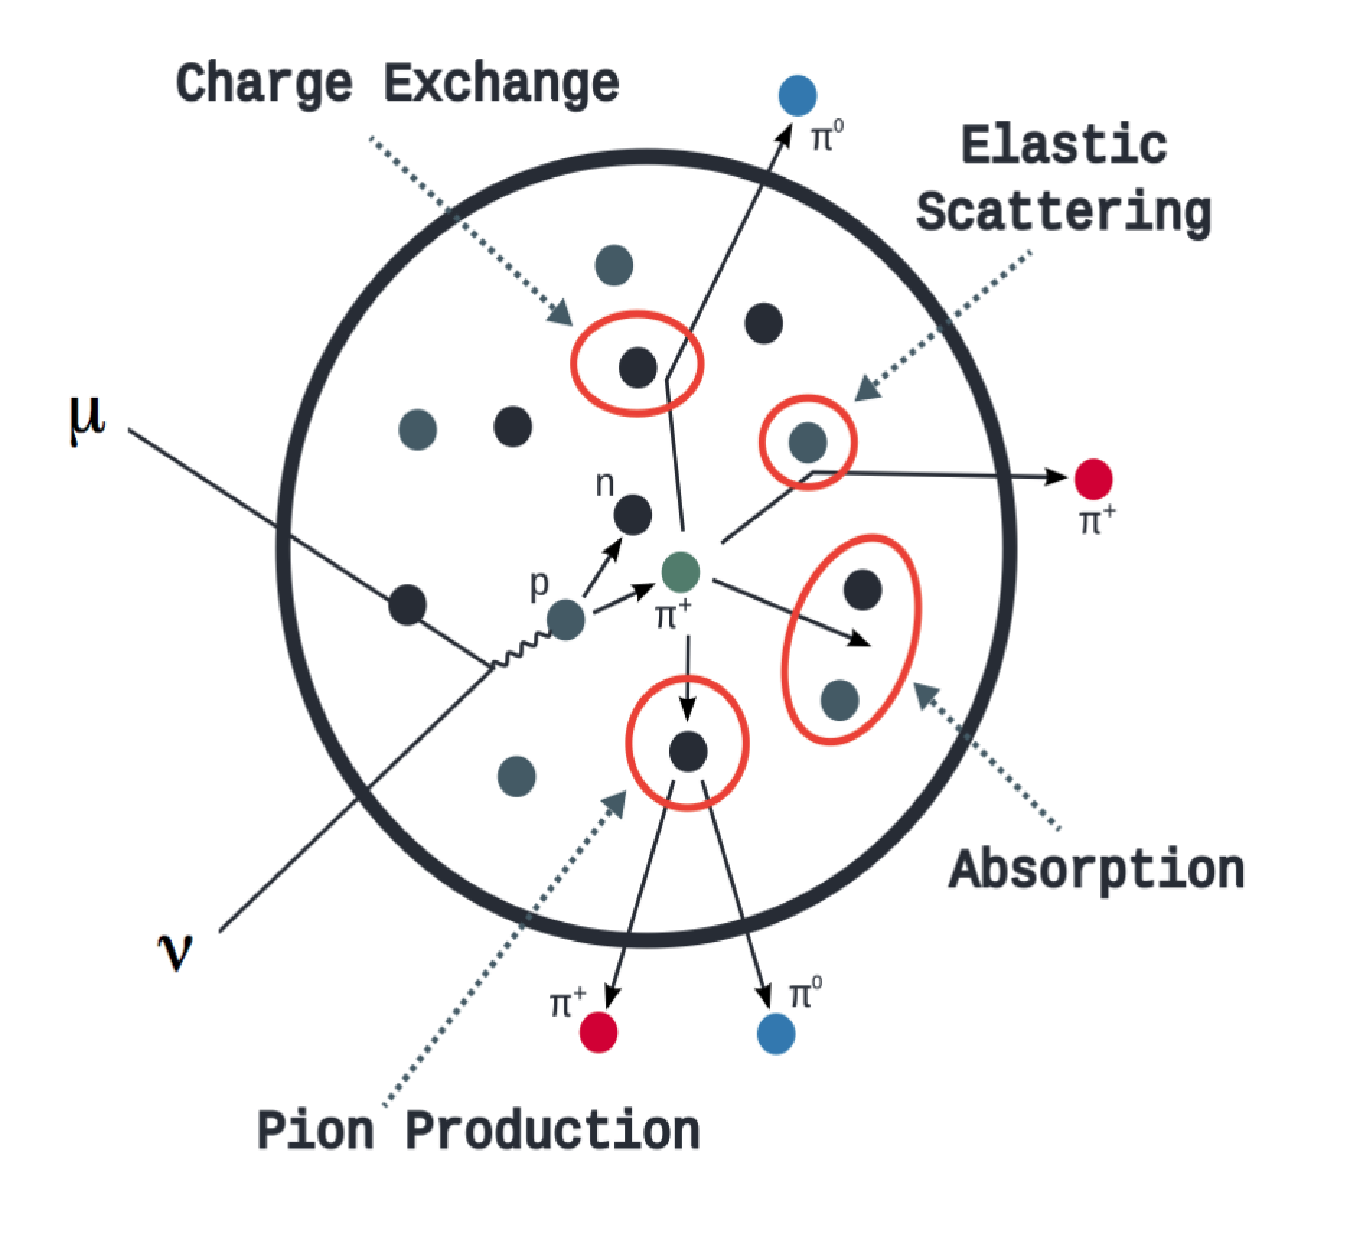
\includegraphics[width=\textwidth, trim={0mm 0mm 0mm 0mm}, clip,page=1]{Figures/Selections/FSIDiagram.pdf}
  \end{subfigure}
  \caption{Illustration of the various processes which a pion can undergo before exiting the nucleus. Taken from \cite{10.48550/arxiv.1602.05299}.}
  \label{fig:Selection_FSIDiagram}
\end{figure}

Any pion which is produced within the nucleus can re-interact through final state interactions before it exits, as illustrated by the scattering, absorption, production and exchange interactions in \autoref{fig:Selection_FSIDiagram}. These re-interactions alter the observable particles within the detector. For instance, if the charged pion from a CC PROD interaction is absorbed, the observables would mimic a CC QE interaction. To simulate these effects, NEUT uses a semi-classical intranuclear cascade model \cite{Hayato2021}. This cascade functions by stepping the pion through the nucleus in fixed-length steps equivalent to \quickmath{dx = R_{N}/100}, where \quickmath{R_{N}} is the radius of the nucleus. At each step, the Monte Carlo allows the pion to interact through scattering, charged exchange, absorption or production with an interaction-dependent probability calculated from a fit to external data \cite{PhysRevD.99.052007}. This cascade continues until the pion is absorbed or exits the nucleus.

Once the outgoing particle kinematics have been determined from NEUT, they are passed into the detector simulation. The near detectors ND280 and INGRID are simulated using a \texttt{GEANT4} package \cite{t2k_det,geant4} to simulate the detector geometry and particle tracking. The response of the detectors is simulated using the elecSim package. The far detector simulation is based upon the original Kamiokande experiment software which uses the \texttt{GEANT3}-based SKDETSIM \cite{Brun:1987ma,t2k_det} package. This controls the interactions of particles in the water as well as Cherenkov light production. The water quality and PMT calibration measurements detailed in \autoref{subsec:T2KSKExp_SKCalibration} are also used within this simulation to make accurate predictions of the detector response.

\section{Event Reconstruction at SK}
\label{sec:Simulation_Reconstruction}

Any above Cherenkov threshold event which occurs in SK will be recorded by the PMT array, where each PMT records the time and accumulated charge it measured. This is shown in the event displays illustrated in \autoref{fig:Selection_SKEventDisplays}. To be useful for physics analyses, this series of PMT hit information needs to be reconstructed to determine the particle's identity and kinematics. This is because the charge and timing distribution of photons generated by a particular particle in an event is dependent upon its initial vertex position, time, direction and momentum of the particle. 

For the purposes of this analysis, the \fq reconstruction algorithm is utilised. Its core function is to compare a prediction of the accumulated charge and timing distribution from each PMT, generated for a particular particle hypothesis, to that observed in the neutrino event. It determines the best particle hypothesis by minimising a likelihood function which includes information from PMTs which were hit and those that were not hit. This improves upon the \texttt{APFit} reconstruction algorithm which has been used for many previous SK analyses. \texttt{APFit} only includes information from PMTs within the \quickmath{43\deg} Cherenkov cone and then sequentially fits the kinematic parameters and particle configuration. Conversely, \fq performs a simultaneous fit, improving both the accuracy of the fit parameters and the rejection of neutral current \quickmath{\pi^{0}} events \cite{Abe2018, Abe2015}. The \fq algorithm is based on the key concepts on the MiniBooNE reconstruction algorithm \cite{Patterson_2009} and described in \cite{t2k_tn_146} which is summarised below.

\begin{figure}[h]
  \begin{subfigure}[t]{0.5\textwidth}
    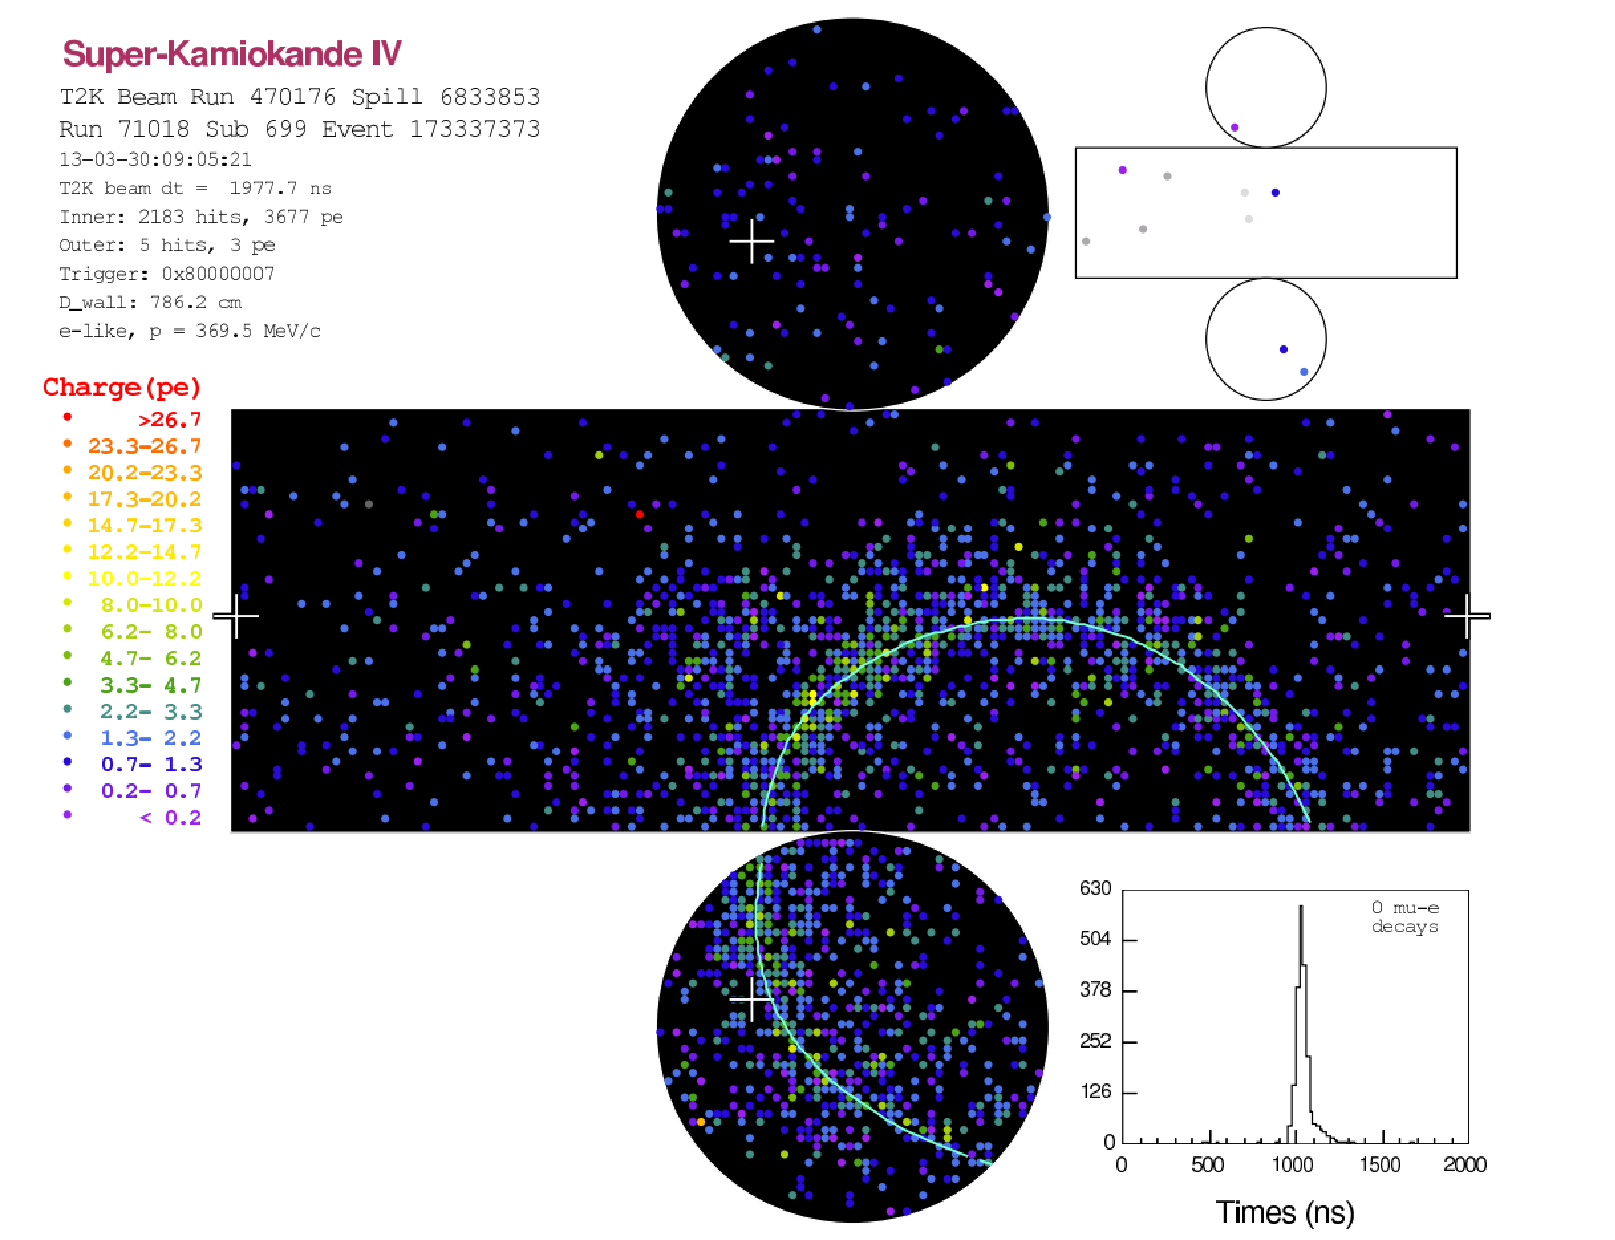
\includegraphics[width=\textwidth, trim={0mm 0mm 0mm 0mm}, clip,page=1]{Figures/Selections/NuECandidate.pdf}
    \subcaption{\quickmath{\nu_{e}}}
  \end{subfigure}%
  \begin{subfigure}[t]{0.5\textwidth}
    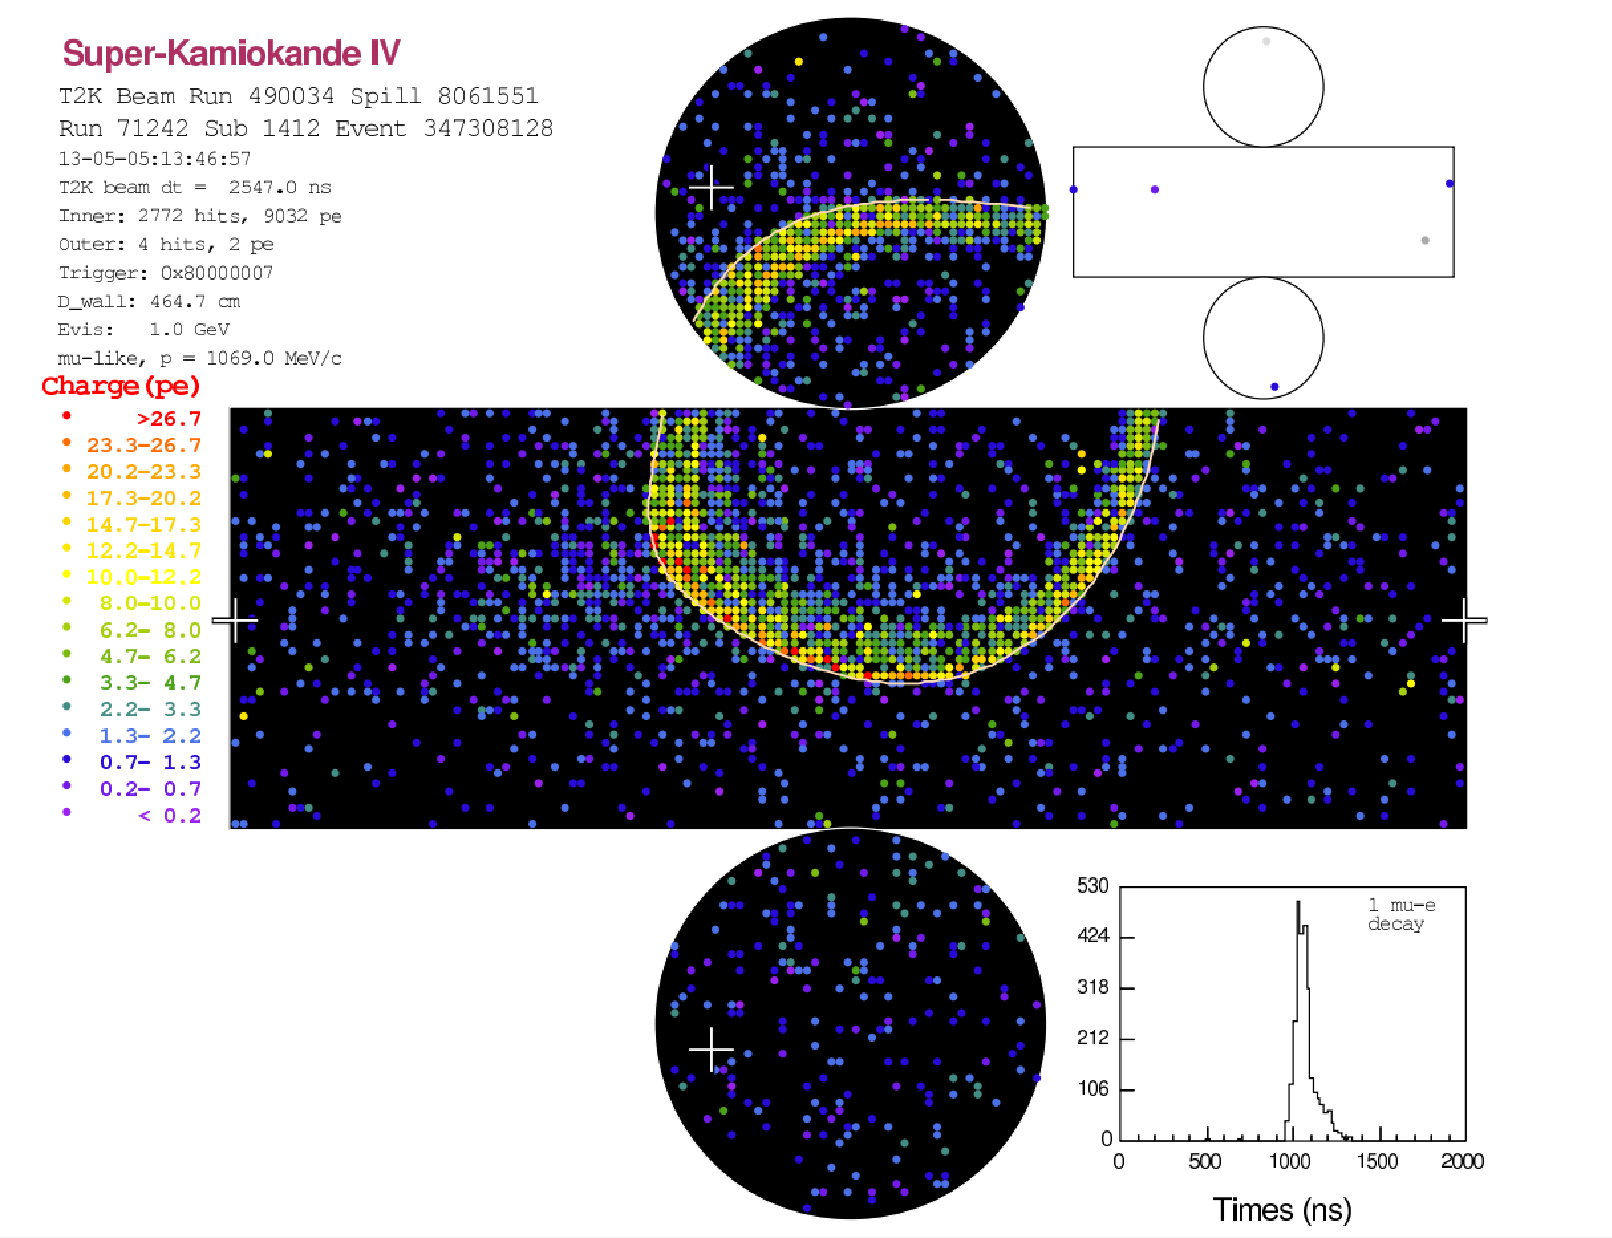
\includegraphics[width=\textwidth, trim={0mm 0mm 0mm 0mm}, clip,page=1]{Figures/Selections/NuMuCandidate.pdf}
    \subcaption{\quickmath{\nu_{\mu}}}
  \end{subfigure}
  \caption{Event displays from Super Kamiokande, illustrating the ``crisp'' ring from a muon and the typically ``fuzzier'' electron ring. Each pixel represents a PMT and thhe color scheme denotes the accumulated charge deposited on that PMT. Figures taken from \cite{t2k_tn_219}.}
  \label{fig:Selection_SKEventDisplays}
\end{figure}

An event in SK can consist of multiple ``sub-events''. For example, a muon neutrino interaction will generate a muon which will subsequently decay to an electron. Both the muon and electron can generate Cherenkov photons but both subevents need to be reconstructed separately. Therefore, to avoid assigning photons generated by the decay-electron to the muon, each event is divided into time clusters, termed ``subevents'', where subevent is defined to contain at most one hit for each PMT. To find the subevents, a vertex goodness metrix is calculated for some vertex position \quickmath{\vec{x}} and time \quickmath{t},

\begin{equation}
  G(\vec{x},t) = \sum^{\texttt{hit PMTs}}_{i} \exp \left( - \frac{1}{2} \left( \frac{T_{Res}^{i}(\vec{x},t)}{\sigma} \right)^{2} \right)
\end{equation}

where

\begin{equation}
  T_{Res}^{i}(\vec{x},t) = t_{i} - t - \left| R^{i}_{PMT} - \vec{x} \right|/c_{n}
\end{equation}

is the residual hit time, \quickmath{R^{i}_{PMT}} is the position of the \quickmath{i^{th}} PMT, \quickmath{c_{n}} is the speed of light in water and \quickmath{\sigma = 4\text{ns}} which is comparable to the time resolution of the PMT. When the fit values of time and vertex are close to the true values, \quickmath{T_{Res}^{i}(\vec{x},t)} tends to zero resulting in subevents appearing as spikes in the goodness metric. The fit vertex and time are grid-scanned, and the values which maximise the goodness metrix are selected as the ``pre-fit vertex''. Whilst this predicts a vertex for use in the clustering algorithm, the final vertex is fit using the higher-precision maximum likelihood method described below.

Once the pre-fit vertex has been determined, the goodness metric is scanned as a function of \quickmath{t} to determine the number of delayed peaks. A peak-finding algorithm is then used on the goodness metric, requiring the goodness metrix to exceed some threshold and drop below a reduced threshold before any delayed additional peaks are considered. The thresholds are set such that the rate of false peak finding is minimised while still attaining good data to Monte-Carlo agreement. To improve performance, the pre-fit vertex for each delayed subevent is re-calculated after PMT hits from the primary subevent are masked. This improves the decay-electron tagging performance. Once all subevents have been determined, the time window around each subevent is then defined by the earliest and latest time which satisfies \quickmath{-180 < T_{Res}^{i} < 800 \text{ns}}. The subevents and associated time windows are then used as seeds for further reconstruction.

For a given subevent, \fq constructs a likelihood based on the accumulated charge \quickmath{q_{i}} and time information \quickmath{t_{i}} from the \quickmath{i^{th}} PMT,

\begin{equation}
  L(\Gamma, \vec{\theta}) = \prod^{\text{unhit}}_{j} P_{j}(\text{unhit}|\Gamma,\vec{\theta}) \prod^{\text{hit}}_{i} \{ 1 - P_{i}(\text{unhit}|\Gamma,\vec{\theta}) \}   f_{q}(q_{i} | \Gamma, \vec{\theta}) f_{t}(t_{i} | \Gamma, \vec{\theta}),
\end{equation}

where \quickmath{\vec{\theta}} defines the track parameters; vertex position, direction vector and momenta, and \quickmath{\Gamma} represents the particle hypothesis. \quickmath{P_{i}(\text{unhit}|\Gamma,\vec{\theta})} defines the probability of the \quickmath{i^{th}} tube to not register a hit given the track parameters and particle hypothesis. The charge likelihood, \quickmath{f_{q}(q_{i} | \Gamma, \vec{\theta})}, and time likelihood, \quickmath{f_{t}(t_{i} | \Gamma,\vec{\theta})}, respresent the probability density function of observing charge \quickmath{q_{i}} and time \quickmath{t_{i}} on the \quickmath{i^{th}} PMT given track parameters \quickmath{\vec{\theta}} and particle hypothesis \quickmath{\Gamma}.

As the generation and propagation of the optical photons is independent of the PMT and electronics response, it is natural to split the calculation into two. Firstly, calculating the expected number of photoelectrons (or predicted charge), \quickmath{\mu_{i}}, at the \quickmath{i^{th}} PMT, and then calculating the likelihood based on this value. This substitution allows the charge likelihood density \quickmath{f_{q}(q_{i} | \mu_{i})} and unhit probability \quickmath{P_{i}(\text{unhit}|\mu_{i})} to be expressed via quantities that are only dependent on the response of the PMT. 

The predicted charge is calculated based on contributions from both the direct light and the scattered light. The direct light contribution is determined based on the integration of the Cherenkov photon profile along the track. PMT angular acceptance and water quality and calibratiion measurements discussed in \autoref{subsec:T2KSKExp_SKCalibration} are included to accurately model the detector's response. The scattered light is calculated in a similar way although it includes a scattering function which depends on vertex of the particle and the position of the PMT. The charge likelihood is calculated by comparing the prediction to the observed charge in the PMT, where the prediction assumes photoelectron generation obeys a Poisson distribution.

The time likelihood is approximated to depend on the vertex \quickmath{\vec{x}}, direction \quickmath{\vec{d}}, and time \quickmath{t} of the track parameters as well as the particle hypothesis. The expected time for PMT hits is calculated by assuming unscattered photons being emitted from the midpoint of the track, \quickmath{S_{mid}},

\begin{equation}
  t^{exp}_{i} = t + S_{mid}/c + |R_{PMT}^{i} - \vec{x} - S_{mid}\vec{d}|/c_{n},
\end{equation}

where \quickmath{c} is the speed of light in vacuum. The time likelihood is then expressed in terms of the residual difference between the PMT hit time and the expected hit time, \quickmath{t^{Res}_{i} = t_{i} - t^{exp}_{i}}. As the first photon hit defines the PMT hit time, the time likelihood density profile is narrower for higher momenta particles which introduces a dependence on the predicted charge. The particle hypothesis and momentum also effect the Cherenkov photon distribution which modifies the shape of the time likelihood density since in reality not all photons are emitted at the midpoint of the track. As with the charge likelihood, the contributions from both the direct and scattered light to the time likelihood density are calculated sparately, which are both calculated from particle gun studies.

The track parameters, \quickmath{\vec{\theta}}, which maximise \quickmath{L(\Gamma | \vec{\theta})} are defined the best fit parameters. In practice MINUIT \cite{James:2296388} is used to minimise the value of \quickmath{-\ln L(\Gamma, \vec{\theta})}. The particle hypothesis is determined by the comparison of  \quickmath{L(\Gamma , \vec{\theta})} across all viable hypotheses, \quickmath{\Gamma}. The fit considers an electron-like, muon-like and charged pion-like hypothesis. The particle's identity is determined by taking the ratio of the liklelihoods of each of the hypotheses. For instance, electrons and muons are distinguished by considering the value of \quickmath{\ln (L_{e}/L_{\mu})} as illustrated in \autoref{fig:Selection_EMUPIDParamDistribution}.

\begin{figure}[h]
  \begin{subfigure}[t]{0.9\textwidth}
    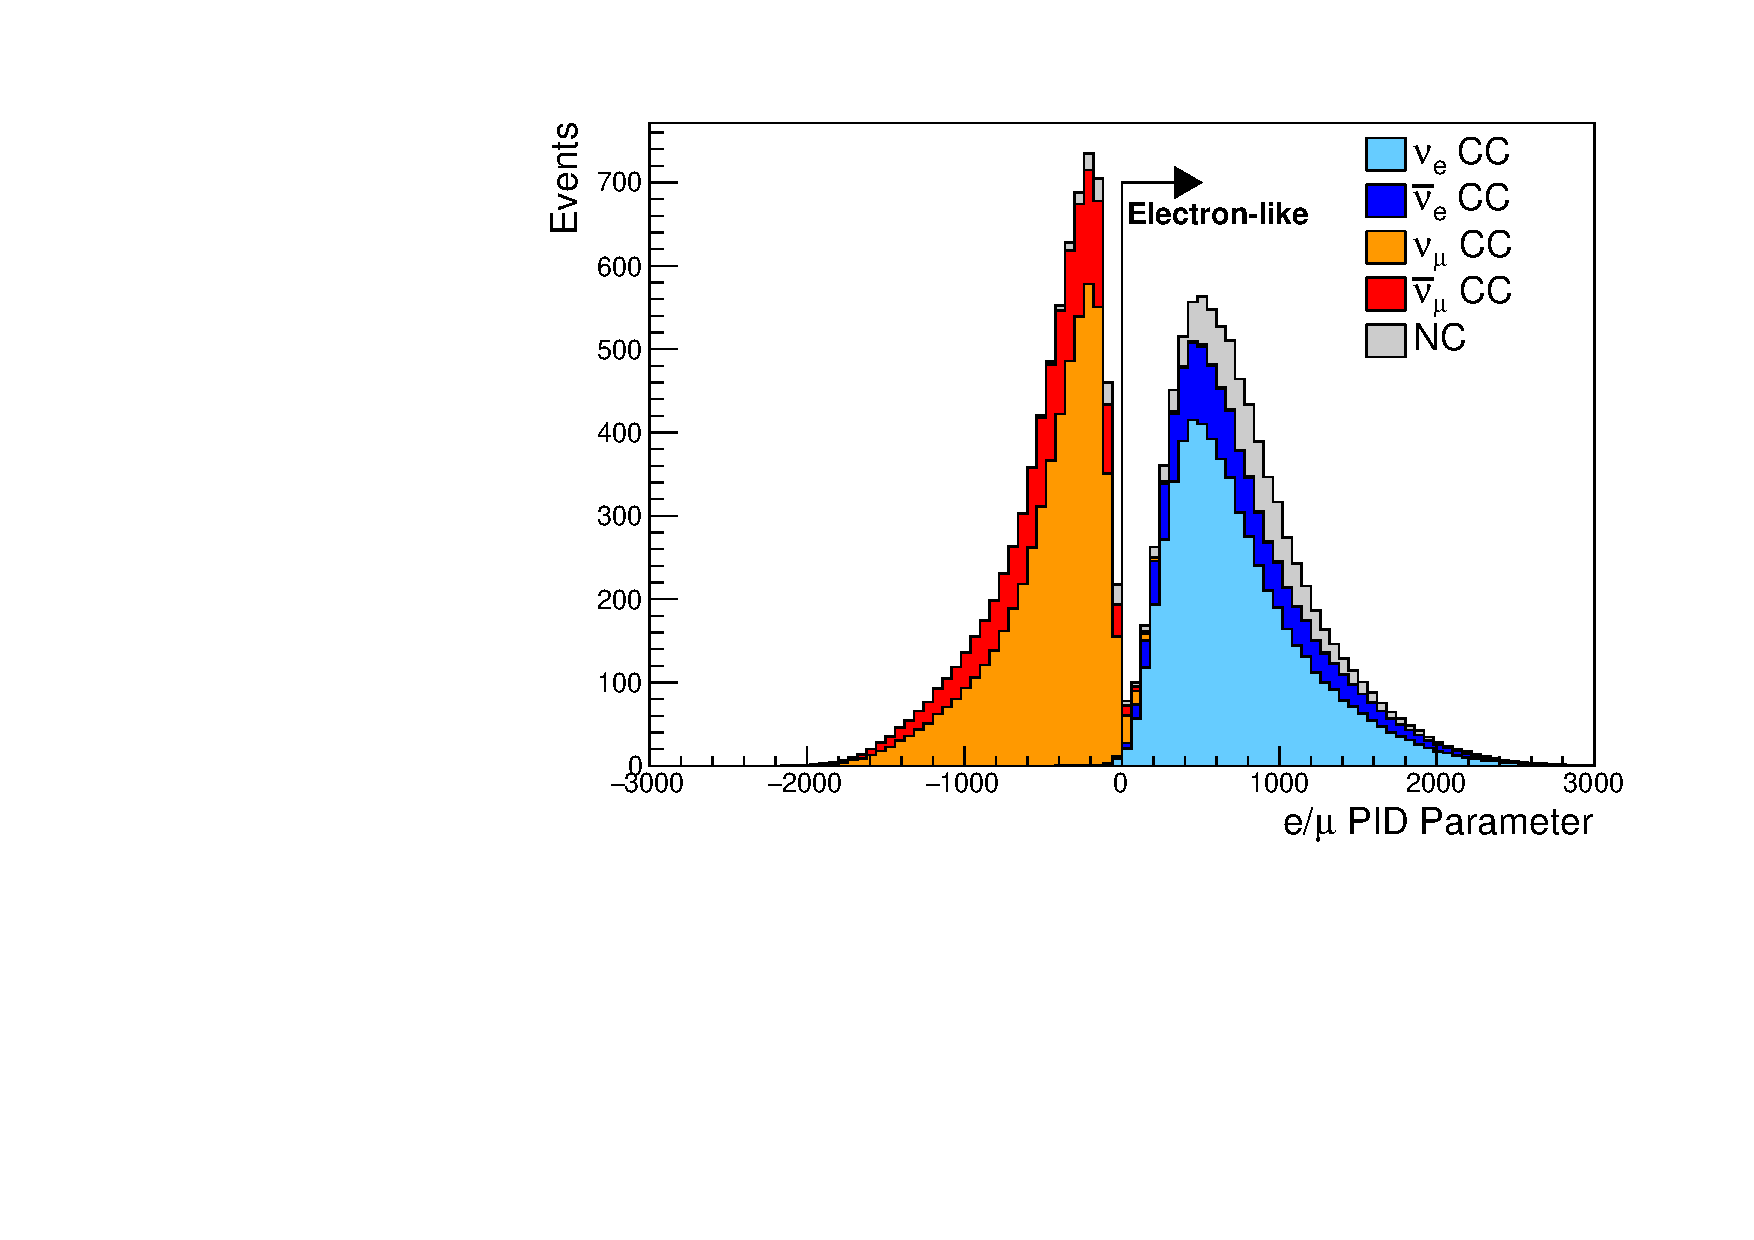
\includegraphics[width=\textwidth, trim={0mm 0mm 0mm 0mm}, clip, page=1]{Figures/Selections/PIDParameter.pdf}
  \end{subfigure}
  \caption{The electron/muon PID separation parameter for all sub-GeV single-ring events in SK-IV. The charged current (CC) component is broken down in four flavours of neutrino (\quickmath{\nu_{\mu}},\quickmath{\bar{\nu}_{\mu}},\quickmath{\nu_{e}} and \quickmath{\bar{nu}_{e}}). Events with positive values of the parameter are determined to be electron-like.}
  \label{fig:Selection_EMUPIDParamDistribution}
\end{figure}

Alongside the three hypotheses which have a single final state particle generating optical photons, denoth ``single-ring'' particle hypotheses. The \fq algorithm also considers a \quickmath{\pi^{0}} hypothesis. To do this, it performs a fit looking for two standard electron-hypothesis tracks which point to the same vertex position and time. This assumes the electron tracks are generated from photon-conversion so the electron tracks actually appear offset from the proposed \quickmath{\pi^{0}} vertex. For these fits, the conversion length, direction and momenta of each photon are also considered as track parameters which are then fit in the same methodoloy as the standard single-ring hypotheses. 

The previous discussion pertains to a single final state particle which generates optical photons. However, the higher energy atmospheric neutrino events can generate finals states with multiple particles which generate Cherenkov photons. These ``multi-ring'' hypotheses are also considered in the \fq algorithm, but only for the first subevent in each ring to reduce computational cost. When calculating the charge likelihood density, the predicted charge associated with each ring is calculated separately and then merged to calculate the total accumulated charge on each PMT. Similarly, the time likelihood for the multi-ring hypothesis is calculated assuming each ring is independent. However, each track is then time ordered based on the time-of-flight from the center of the track to the PMT, and the direct light from any ring is inicident on the PMT arrives before any scattered light. To reduce computational resources required for a fit, the multi-ring fits only consider electron-like and charged pion-like rings as the pion fit can be used as a proxy for a muon fit due to their similar mass.

Typically, multi-ring fits have the largest likelihood because of the additional degrees of freedom introduced. Multi-ring fits proceed by proposing another ring to the previous fit and then fitting the parameters in the method described above. The additional ring is only added if the ratio of likelihoods between the \quickmath{n} and \quickmath{n+1} passes a criteria. The criteria values for single-ring and multi-ring separation have been determined to be \quickmath{9.35}(\quickmath{11.83}) based on Monte-Carlo studies, for hypotheses with electron-like(muon-like) first ring.

As an example of how the reconstruction depends on the detector conditions, the author of this thesis assessed the quality of event reconstruction for SK-V data. The detector systematics invoked within the T2K-only oscillation analysis are determined using data to Monte Carlo comparisons using the SK-IV data \cite{t2k_tn_326}. Due to tank-open maintanence occuring between SK-IV and SK-V, the dark rate of each PMT was observed to increase due to light exposure for a significant time during the repairs. This can be seen in \autoref{fig:Selection_DarkRateVariation}. Run-10 of the T2K experiment was conducted in the SK-V period, so the consistency of SK-IV and SK-V data needs to be studied to determine whether the SK-IV defined systematics can be applied to the run-10 data. This study was performed using the stopping muon data set for both the SK-IV and SK-V periods. This data is used due to the high rate of interactions, \quickmath{O(200)} events per hour, as well as having similar energies to muons from CCQE \quickmath{\nu_{\mu}} interactions. The rate of cosmic muons does depend on the solar activity cycle \cite{Maghrabi2021}. This has been neglected in this comparison study as it is the shape of the distibutions which is important for the purposes of being compared to the detector systematics. \quickmath{2398.42} and \quickmath{626.719} hours of SK-IV and SK-V are used which equates to \quickmath{686743} and \quickmath{192504} events respectively.

\begin{figure}[h]
  \begin{subfigure}[t]{\textwidth}
    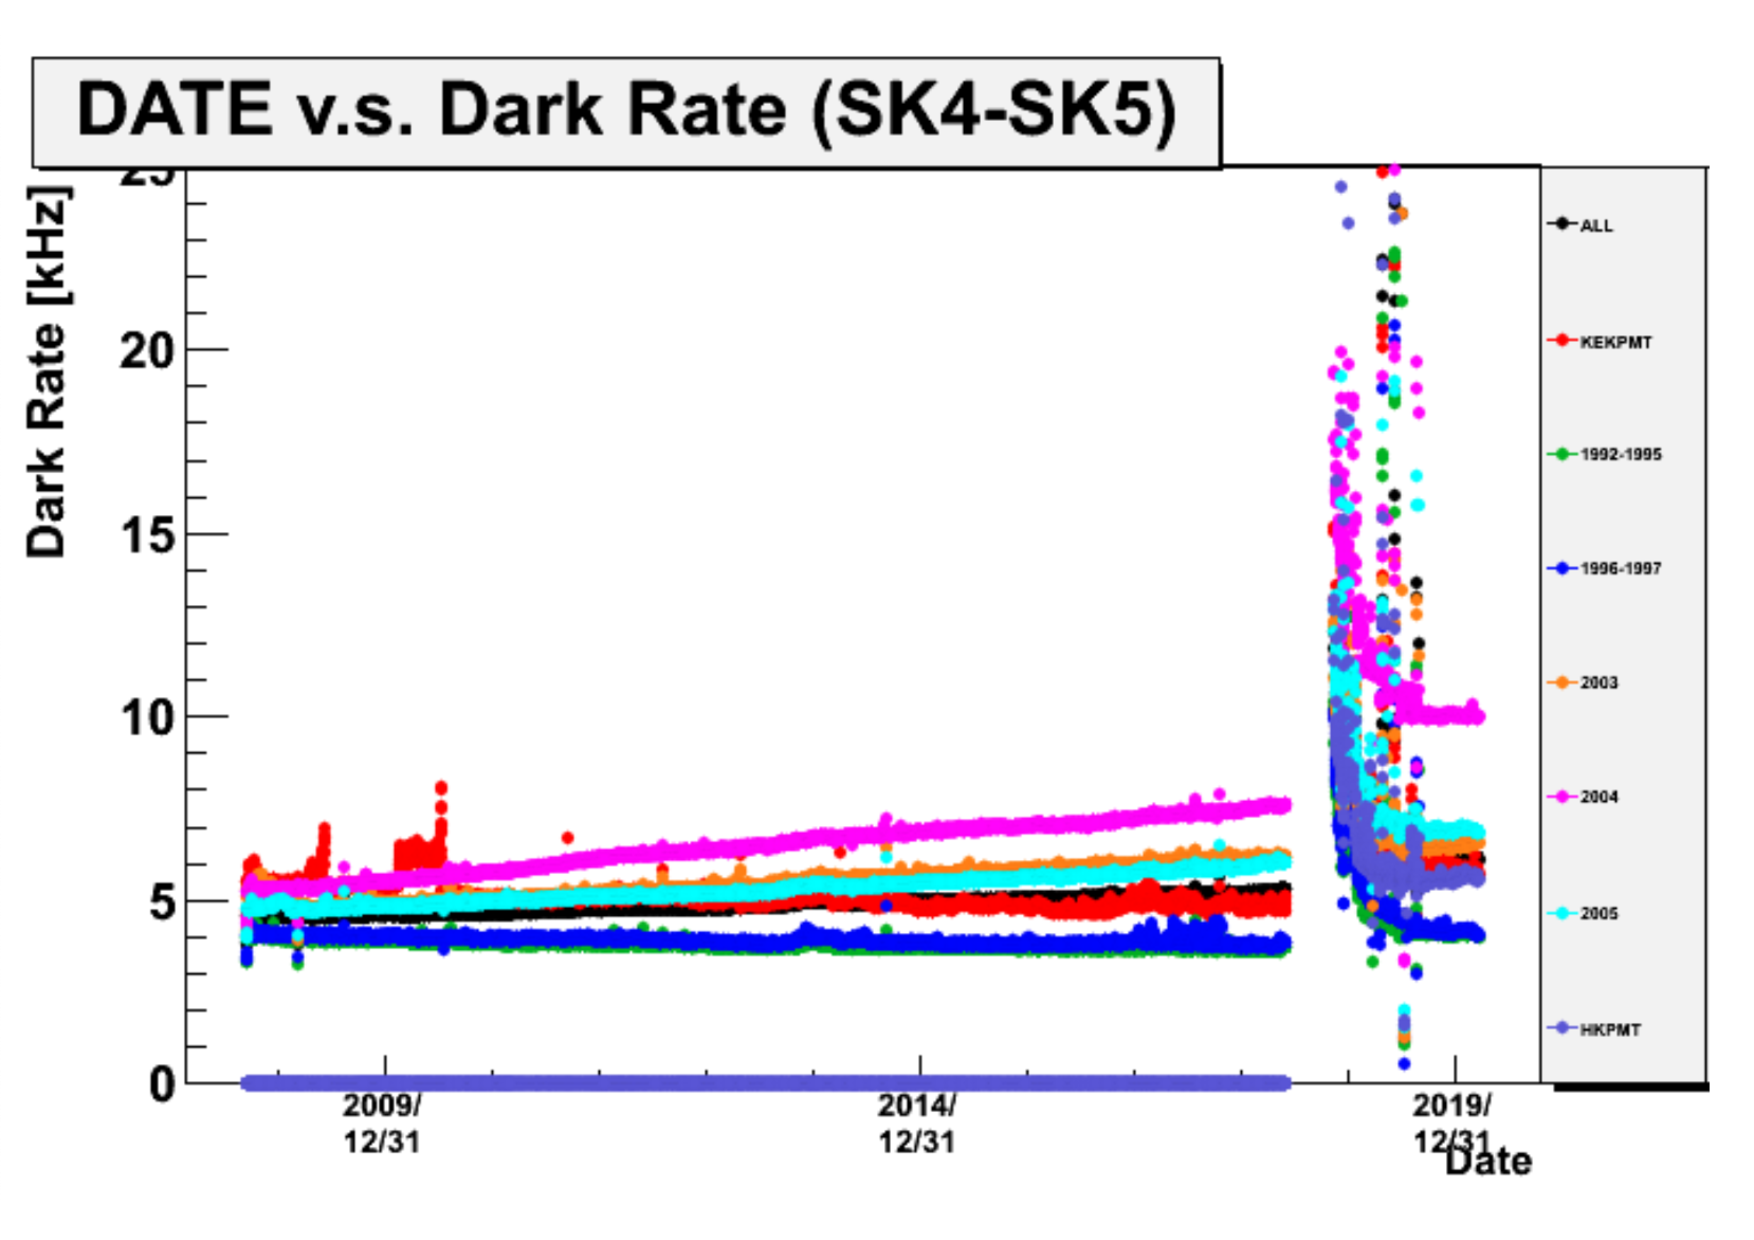
\includegraphics[width=\textwidth, trim={0mm 0mm 0mm 0mm}, clip, page=1]{Figures/Selections/DarkRate.pdf}
  \end{subfigure}
  \caption{The variation of measured dark rate as a function of date, broken down by PMT type. The SK-IV and SK-V periods span September 2008 to May 2018 and January 2019 to July 2020 respectively. The break in measurement between 2018 corresponds to the period of tank repair and refurbishment. Figure adapted from \cite{t2k_tn_326}.}
  \label{fig:Selection_DarkRateVariation}
\end{figure}

The predicted charge used in the \fq charge likelihood calculation for each PMT includes the photoelectron emission contribution from the dark rate of the PMT. Therefore, the increase in dark rate needs to be accounted for. In practice, the reconstruction algorithm takes the average dark rate for all PMTs for each SK period as an input and predicts the associated charge from this contribution. The dark rate was calculated by averaging the dark rate per run for each period separately, using the calibration measurements detailed in \autoref{subsec:T2KSKExp_SKCalibration}. The average dark rate from SK-IV and SK-V were found to be \quickmath{4.57kHz} and \quickmath{6.30kHz}, respectively. The associated charge with the muon and decay electron subevents are illustrated in \autoref{fig:Selection_MeasuredChargeDistribution}. As expected, the increase in dark rate is not observed in the muon subevent which is of typically higher energy. However it has a clear effect on the decay electron subevent which is lower energy.

\begin{figure}[h]
  \begin{subfigure}[t]{0.48\textwidth}
    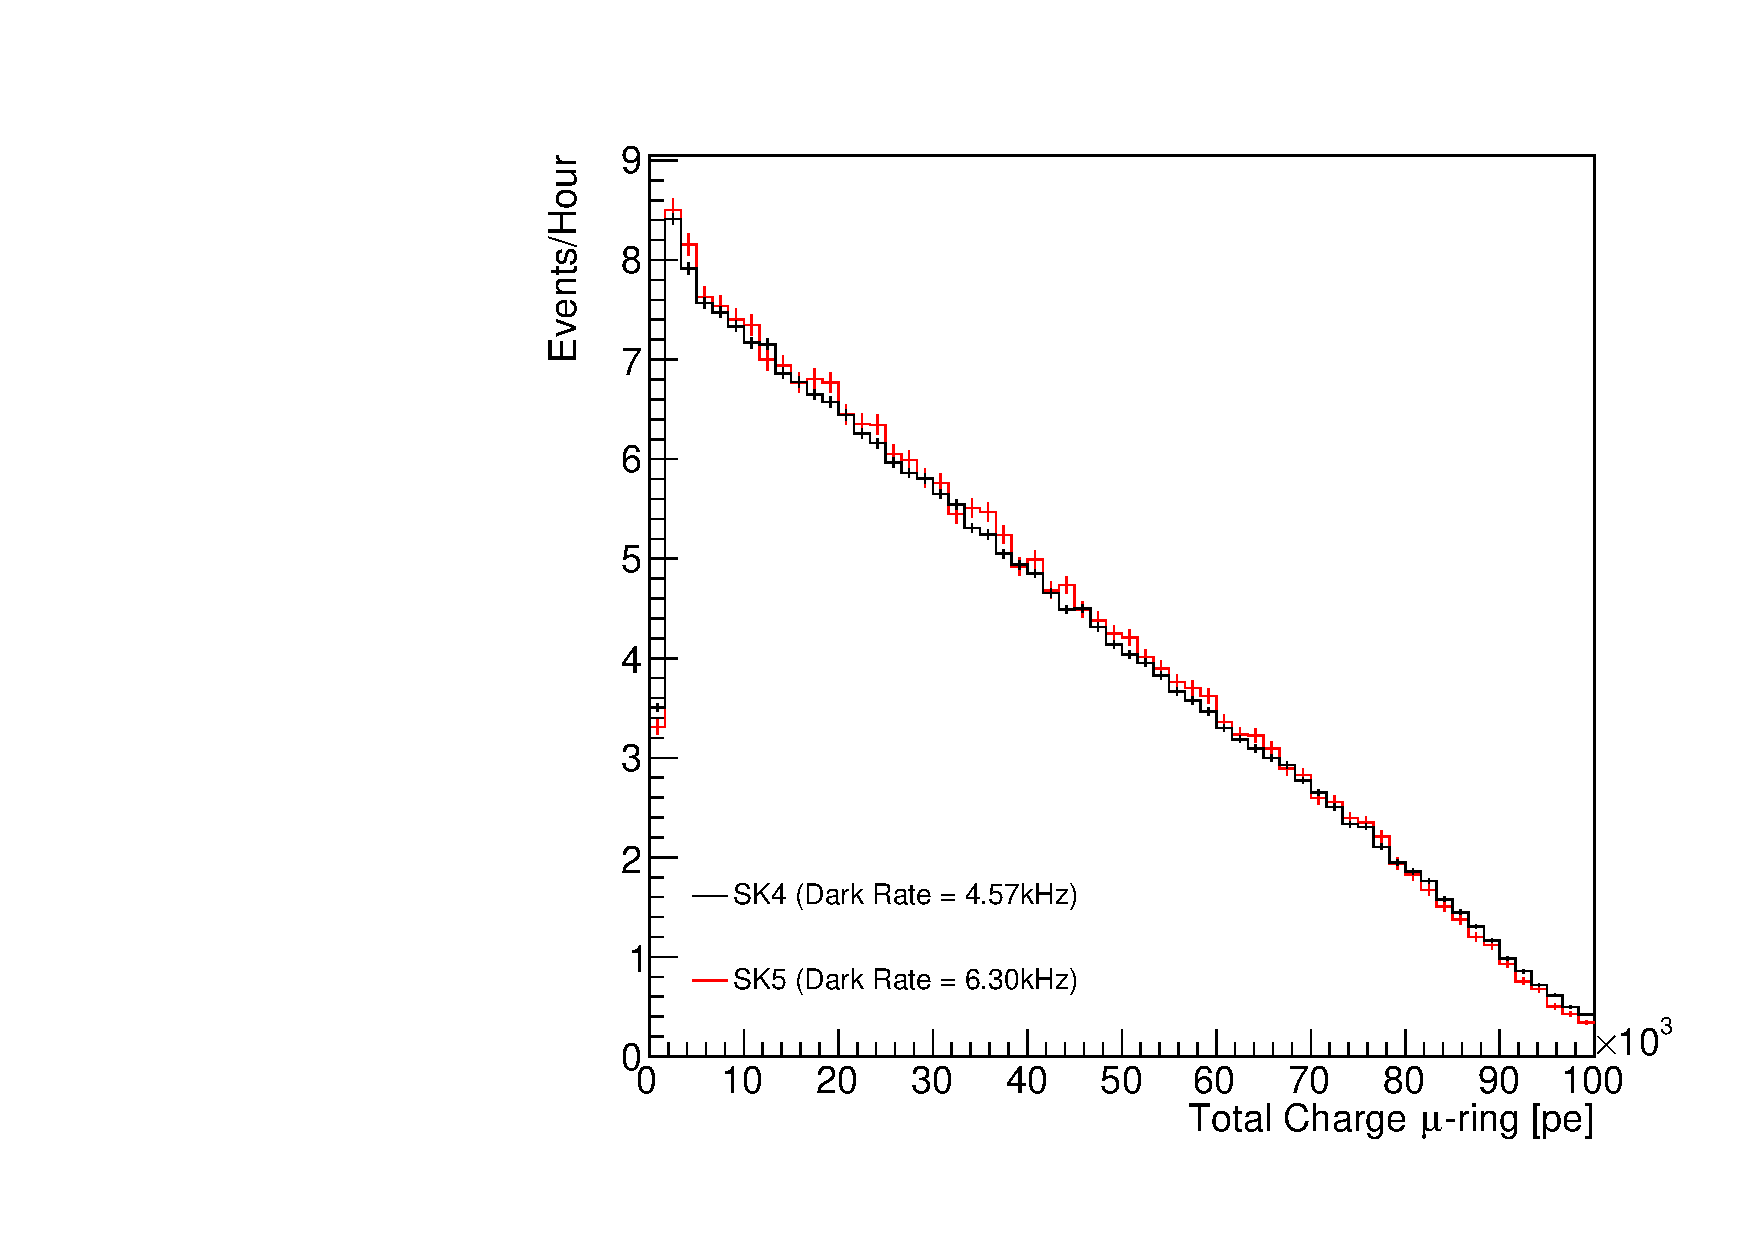
\includegraphics[width=\textwidth, trim={0mm 0mm 0mm 0mm}, clip, page=1]{Figures/Selections/ChargeAssociatedWithMuon.pdf}
    \subcaption{Muon}
  \end{subfigure}%
  \begin{subfigure}[t]{0.48\textwidth}
    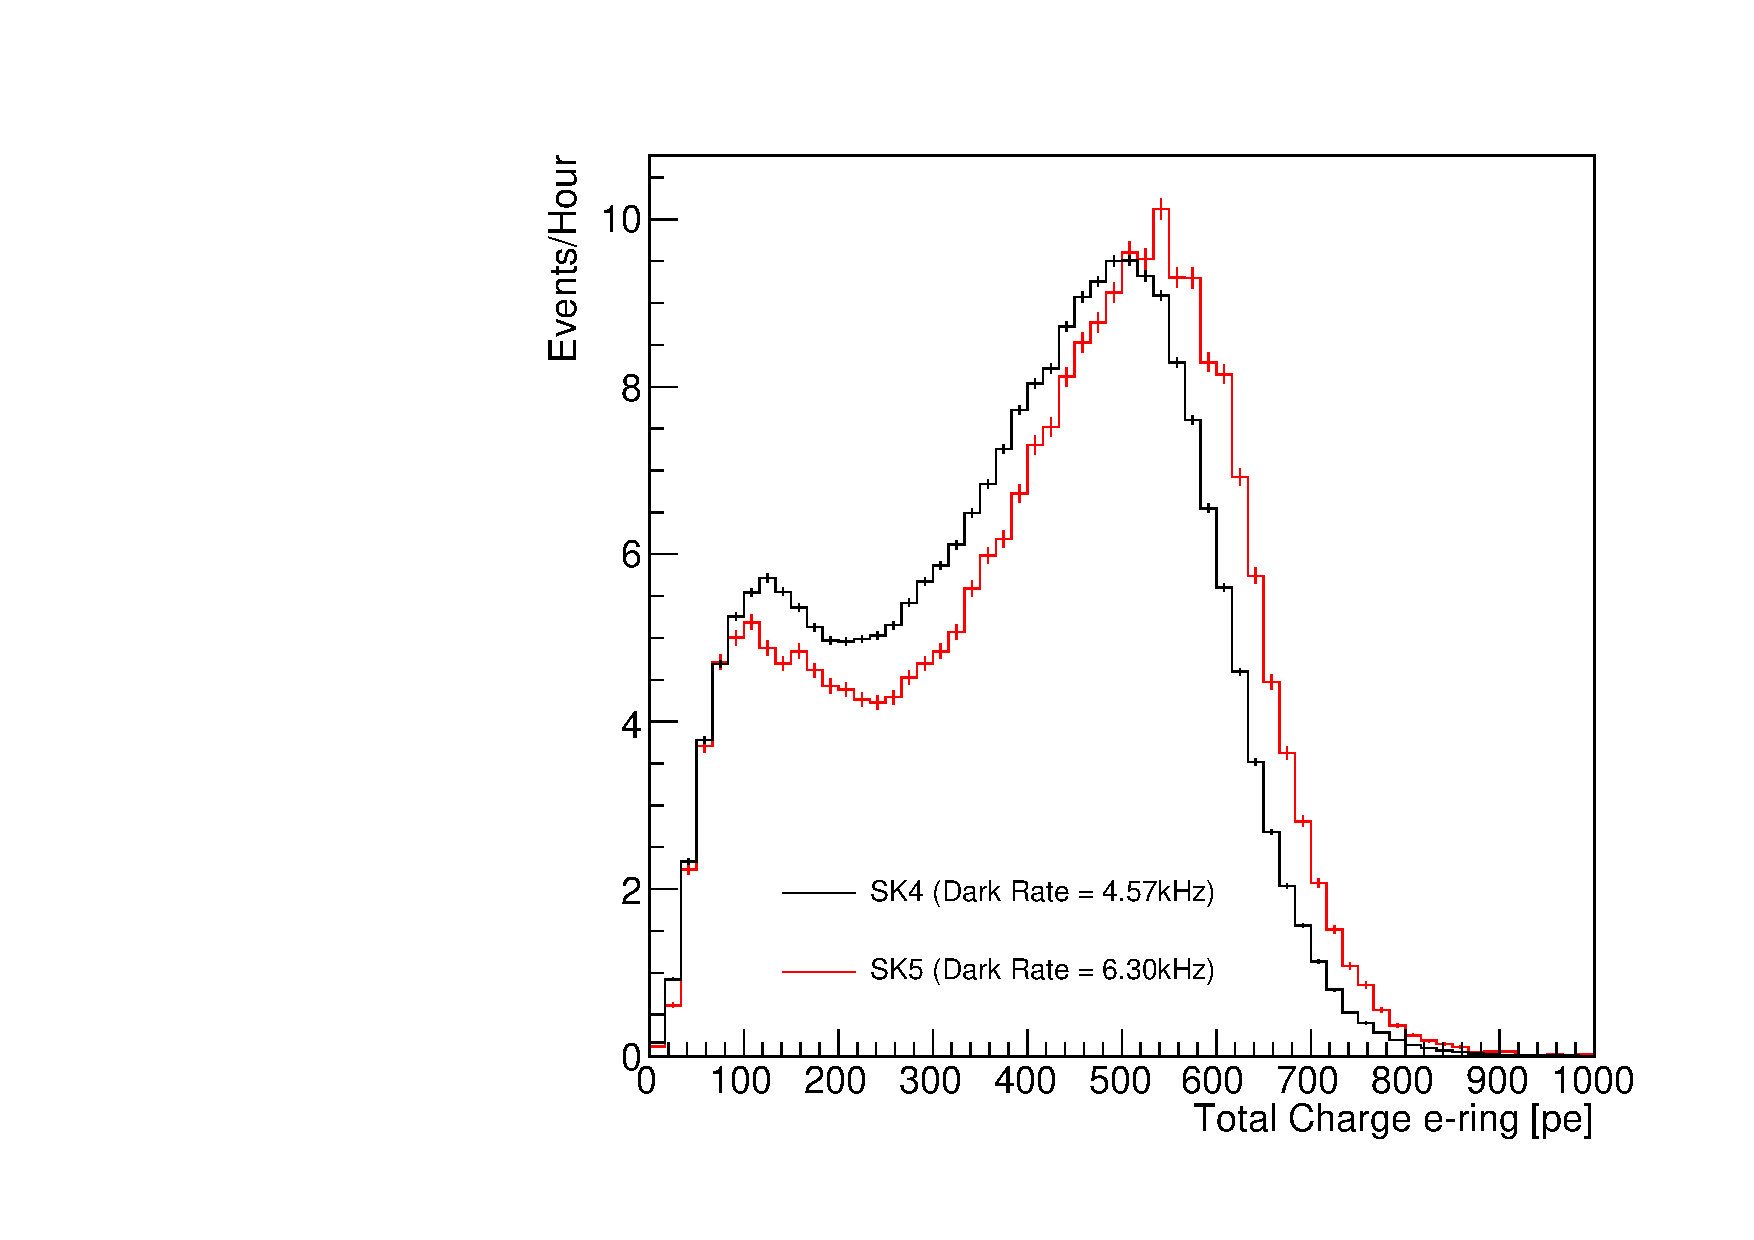
\includegraphics[width=\textwidth, trim={0mm 0mm 0mm 0mm}, clip, page=1]{Figures/Selections/ChargeAssociatedWithDecayE.pdf}
    \subcaption{Decay Electron}
  \end{subfigure}  
  \caption{Comparison of the measured raw-charge deposited per event from the stopping muon data samples between SK-IV (Blue) and SK-V (Red), split by the primary muon subevent and the associated decay electron subevent.}
  \label{fig:Selection_MeasuredChargeDistribution}
\end{figure}

The energy scale systematic for the SK-IV period was determined to be \quickmath{2.1\%} \cite{sk_2017}. It is defined to be equal to the difference between data and Monte Carlo prediction in the stopping muon data sample. To determine the consistency of the SK-IV and SK-V with respect to the energy scale systematic, the muon momentum distribution is compared between the two SK periods. The distribution of Cherenkov photons is dependent upon on the momentum of the particle. This is then integrated along the track length of the particle to determine the PMT hit probability for each PMT. Consequently, the reconstructed momentum divided by track length is compared between SK-IV and SK-V as illustrated in \autoref{fig:Selection_MuonMomentumByRange}.

\begin{figure}[h]
  \begin{subfigure}[t]{\textwidth}
    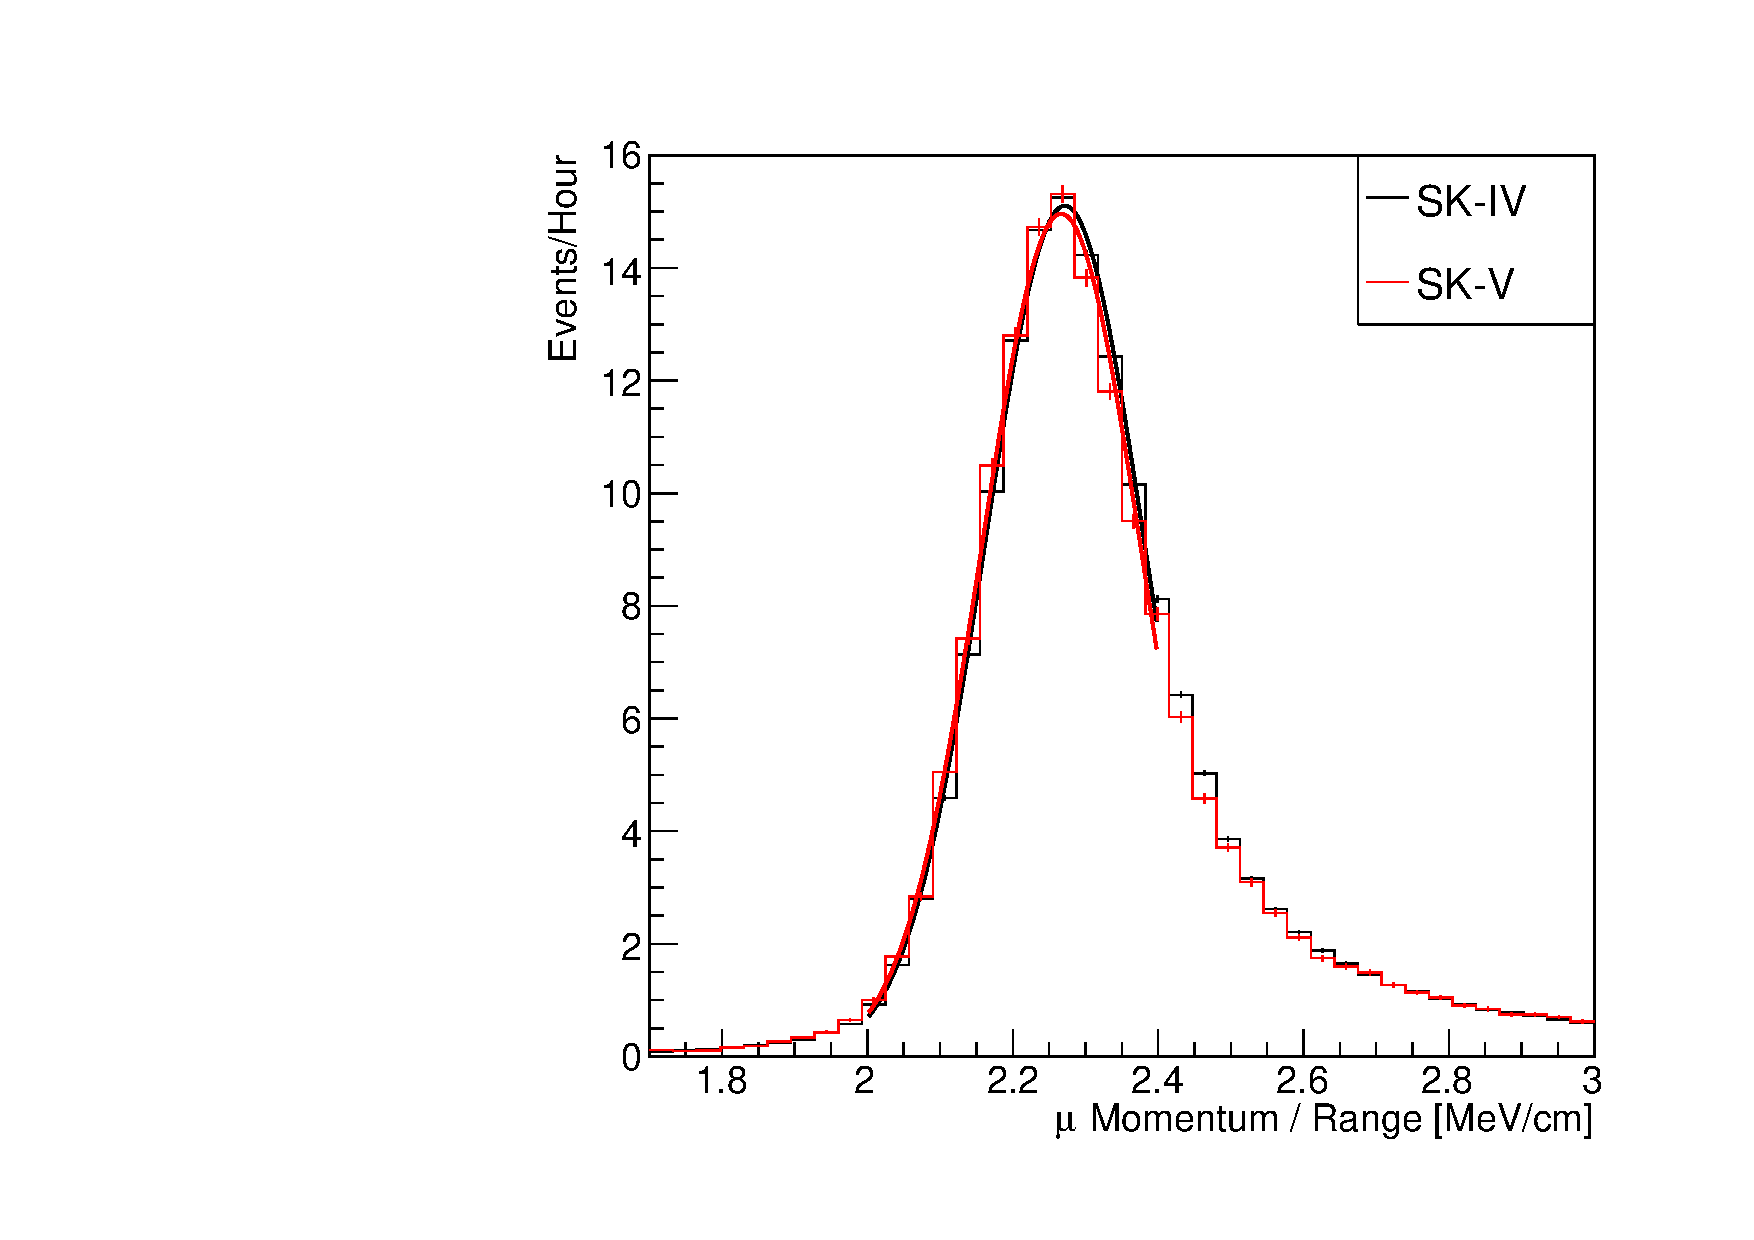
\includegraphics[width=\textwidth, trim={0mm 0mm 0mm 0mm}, clip, page=1]{Figures/Selections/MuonRangeComparison.pdf}
  \end{subfigure}
  \caption{The distribution of the reconstructed momentum from the muon ring divided by the distance between the reconstructed muon and decay electron vertices as found in the stopping muon data sets of SK-IV (Black) and SK-IV (Red). Only events with one tagged decay electron and considered. A Gaussian fit is considered in the range \quickmath{[2.0,2.4] \text{MeV/cm}} and illustrated as the solid curve.}
  \label{fig:Selection_MuonMomentumByRange}
\end{figure}

The consistency between these distributions has been computed in two ways. Firstly, a Gaussian is fit to each distribution separately. The mean of which is found to be \quickmath{(2.272 \pm 0.003) \text{MeV/cm}} and \quickmath{(2.267 \pm 0.006) \text{MeV/cm}} for SK-IV and SK-V respectively. The ratio of these is equal to \quickmath{1.002 \pm 0.003}. The mean of the Gaussian's is consistent with the expected stopping power of a minimum ionising muon for a target material (water) with \quickmath{Z/A \sim 0.5} \cite{PhysRevD.86.010001}. The secod consistency check is performed by introducing a nuisance parameter, \quickmath{\alpha}, which modifies the SK-V distribution. The value of \quickmath{\alpha} which minimises the \quickmath{\chi^{2}} between the SK-IV and SK-V is determined by scanning across a range of values. This is repeated by applying \quickmath{\alpha} as a multiplicative factor and an additive shift. The \quickmath{\chi^{2}} distributions for different values of \quickmath{\alpha} is illustrated in \autoref{fig:Selection_MuonMomentumByRangeChi2Scan}. The values which minimise the \quickmath{\chi^{2}} are found to be \quickmath{0.0052} and \quickmath{1.0024} for the additive and multiplicative implementations respectively. No evidence of shifts larger than the \quickmath{2.1\%} uncertainty on the energy scale systematic have been found in the reconstructed momentum distribution of SK-IV and SK-V.

\begin{figure}[h]
  \begin{subfigure}[t]{\textwidth}
    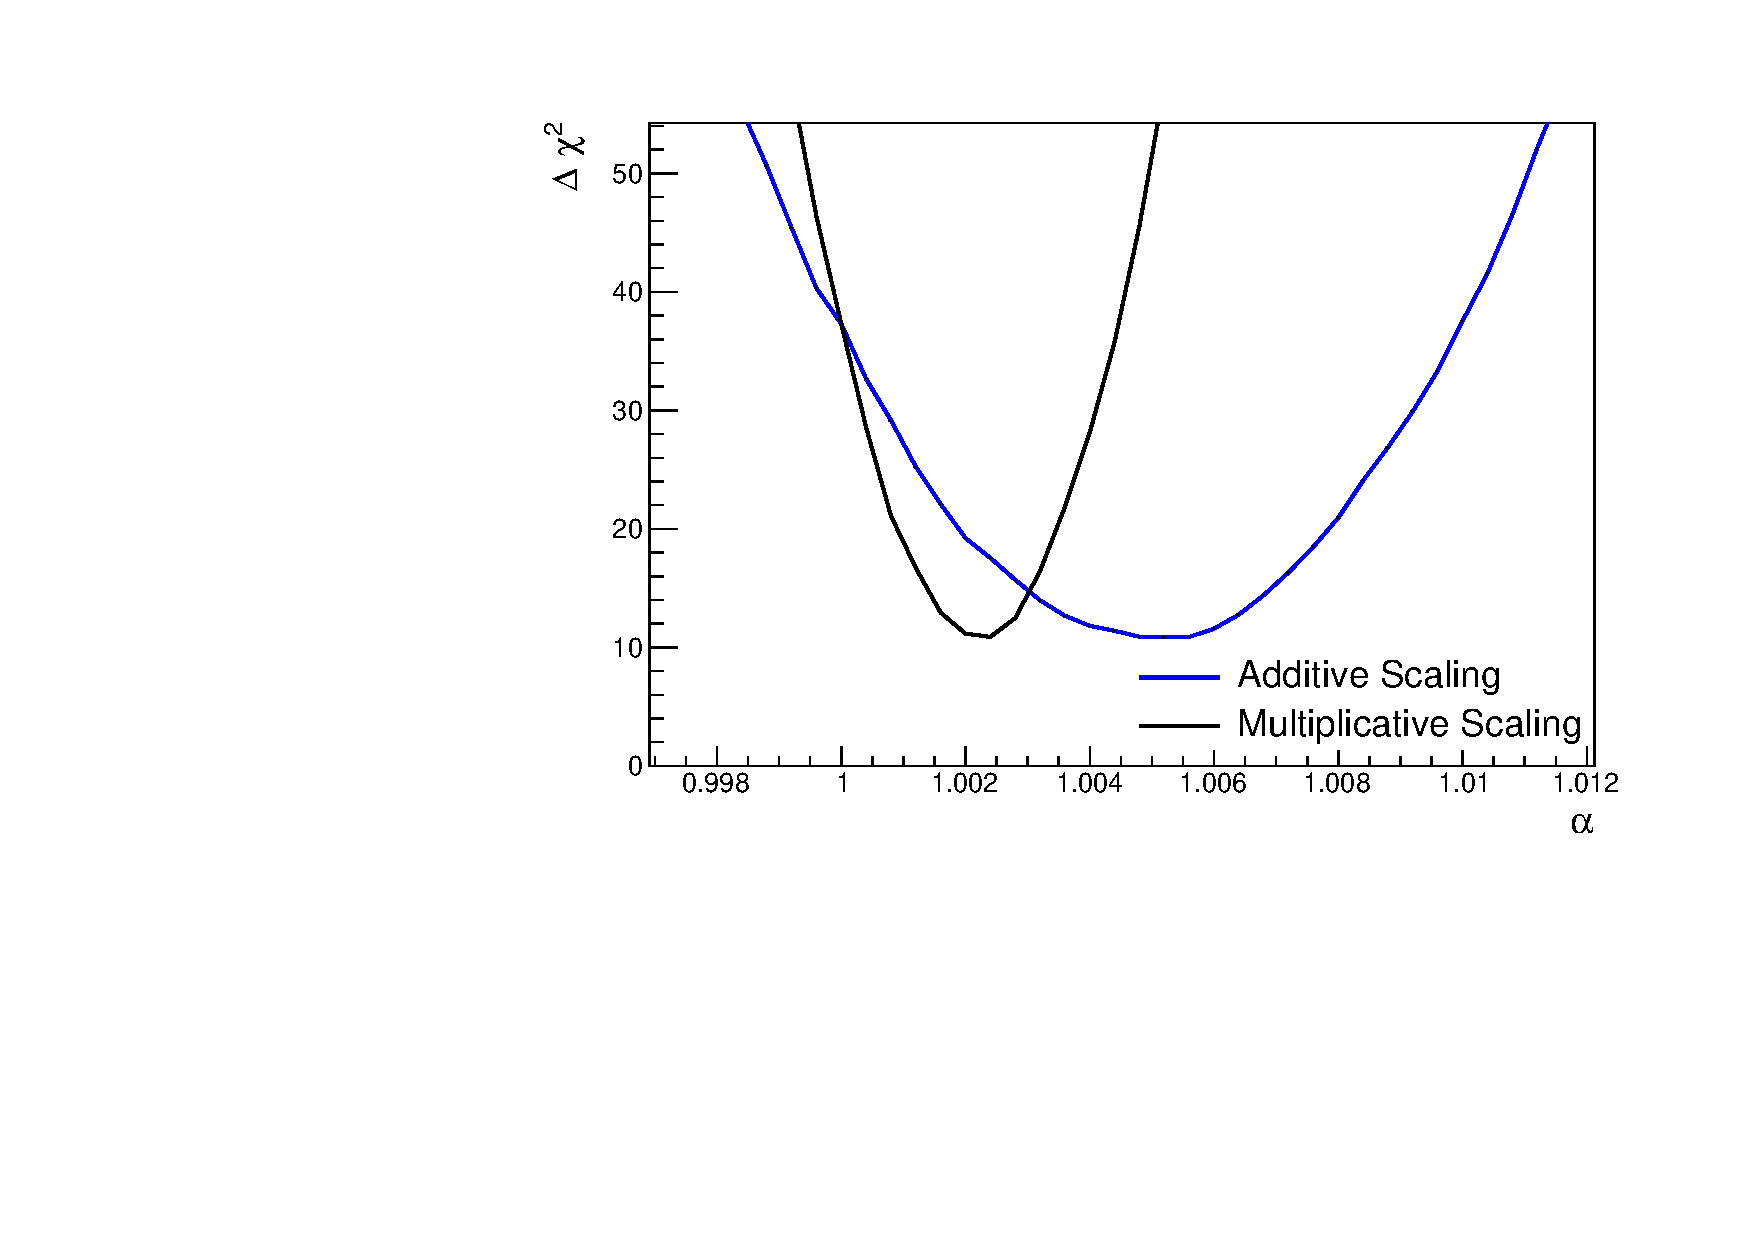
\includegraphics[width=\textwidth, trim={0mm 0mm 0mm 0mm}, clip, page=1]{Figures/Selections/MuonRange_Chi2Scan.pdf}
  \end{subfigure}
  \caption{The \quickmath{\chi^{2}} difference between the SK-IV and SK-V reconstructed muon momentum divided by range when the SK-V is modified by the scaling parameter \quickmath{\alpha}. Both additive (Blue) and multiplicative (Black) scaling factors have been considered. In practice, the additive scaling factor actually uses the value of (\quickmath{\alpha-1.0}).}
  \label{fig:Selection_MuonMomentumByRangeChi2Scan}
\end{figure}

\section{Event Selection at SK}
\label{sec:Selections_Selection}
